%!TEX TS-program = xelatex
% !Mode:: "TeX:UTF-8"
\documentclass[a4paper]{article}
\usepackage[margin=2cm]{geometry}
\usepackage{amsmath,amssymb,amsthm}
\renewcommand{\baselinestretch}{1.67}
\pagestyle{empty}
\usepackage{xeCJK}
                     \setCJKfamilyfont{heiti}{黑体}                        %偶iC只用两字体,黑体和Adobe宋体,字号用了三号和四号,其余多余
                     \newcommand{\heiti}{\CJKfamily{heiti}}
%                     \setCJKfamilyfont{kaishu}{楷体}
%                     \newcommand{\kaishu}{\CJKfamily{kaishu}}
%                     \setCJKfamilyfont{songti}{宋体}
%                     \newcommand{\songti}{\CJKfamily{songti}}
\setCJKmainfont{Adobe Song Std}
%\newcommand{\chuhao}{\fontsize{42.2pt}{\baselineskip}\selectfont}     % 初号
%\newcommand{\Chuhao}{\fontsize{36.1pt}{\baselineskip}\selectfont} % 小初号
%\newcommand{\yihao}{\fontsize{26.1pt}{\baselineskip}\selectfont}      %一号
%\newcommand{\Yihao}{\fontsize{24.1pt}{\baselineskip}\selectfont}      %小一号
%\newcommand{\erhao}{\fontsize{22.1pt}{\baselineskip}\selectfont}      %二号
%\newcommand{\Erhao}{\fontsize{18.1pt}{\baselineskip}\selectfont}  %小二号
\newcommand{\sanhao}{\fontsize{16.1pt}{\baselineskip}\selectfont}  % 三号
\newcommand{\sihao}{\fontsize{14.1pt}{\baselineskip}\selectfont}%     四号
%\newcommand{\Sihao}{\fontsize{12.1pt}{\baselineskip}\selectfont}  %小四号
%\newcommand{\wuhao}{\fontsize{10.0pt}{\baselineskip}\selectfont}    %五号
%\newcommand{\Wuhao}{\fontsize{9.0pt}{\baselineskip}\selectfont}   %小五号
%\newcommand{\liuhao}{\fontsize{7.5pt}{\baselineskip}\selectfont}  % 六号
%\newcommand{\qihao}{\fontsize{5.5pt}{\baselineskip}\selectfont}    % 七号
\usepackage{pifont}                                                                                                                  %编号圈1到圈10
\usepackage[perpage,symbol*]{footmisc}                                                                                %编号圈1到圈10
\DefineFNsymbols{circled}{{\ding{192}}{\ding{193}}{\ding{194}}
                                            {\ding{195}}{\ding{196}}{\ding{197}}{\ding{198}}
                                            {\ding{199}}{\ding{200}}{\ding{201}}}\setfnsymbol{circled}          %编号圈1 到圈10
%\usepackage{esvect}%向量\vv
%\usepackage{upgreek}
\usepackage{graphicx,picinpar}   % picinpar 是用来调整图片位置的等等,用tikz后,这些多余
\usepackage{tikz}
\begin{document}

\begin{center}
\linespread{1}\selectfont {\heiti \sihao 2013年4月查漏补缺文理合卷}\par {\heiti \sanhao 高二下数学}    %选修2-1,选修2-2; 选修1-1,选修1 -2
\end{center}



{\heiti 附:随机变量$\boldsymbol K^2$的概率分布}
\begin{center}
\linespread{1.25}\selectfont
\begin{tabular}{|c|c|c|c|c|c|c|c|c|c|c|}
  \hline
             $P(K^2\ge k)$   & 0.50     &0.40      & 0.25     &0.15    & 0.10      &0.05      &0.025    & 0.010     &0.005      &0.001 \\
  \hline
             $k$                   & 0.455   & 0.708   & 1.323   & 2.072 & 2.706    & 3.841   & 5.024   & 6.635     & 7.879     & 10.828 \\
  \hline
\end{tabular}
\end{center}

\smallskip



\begin{enumerate}
\item  $\mathrm{i}$是虚数单位,$n$是正整数,则$\mathrm{i}^n+\mathrm{i}^{n+1}+\mathrm{i}^{n+2}+\mathrm{i}^{n+3}=$\underline{\hbox to 15mm{}}.






\item  (文科)在研究身高和体重的关系时,求得相关指数$R^2\approx$\underline{\hbox to 10mm{}},可以叙述为“身高解释了64\% 的体重变化,而随机误差贡献了剩余的36\%” 所以身高对体重的效应比随机误差的效应大得多.

  (理科)函数$f(x)=\sqrt{x}$的图象在$x=4$处的切线方程是\underline{\hbox to 15mm{}}.








\item  (文科)某高校“统计初步”课程的教师随机调查了选该课的一些学生情况,具体数据如下表:
\begin{center}
\linespread{1.25}\selectfont
\begin{tabular}{|c|c|c|}
  \hline
            性别 & 非统计专业   &统计专业\\
  \hline
            男     & 13   &10\\
  \hline
            女        & 7   &20 \\
  \hline
\end{tabular}
\end{center}

为判断主修统计专业是否与性别有关系,根据表中数据得到${k=\dfrac{50\times(13\times20-10\times7)^2}{23\times27\times20\times30}\approx 4.844}$,因为\underline{\hbox to 15mm{}},所以判定主修统计专业与性别\underline{\hbox to 10mm{}} (填空“有”或“无”)关系,那么这种判断出错的可能性为\underline{\hbox to 10mm{}}.

          (理科)设函数$f(x) = x\ln x,x \in [\mathrm{e}^{ - 2},\mathrm{e}]$,则$f(x)\) 的最大值为\underline{\hbox to 15mm{}},最小值为\underline{\hbox to 15mm{}}.






\item  (文科)某工厂的某种型号的机器的使用年限$x$和所支出的维修费用$y$ (万元)有下表的统计资料:
\begin{center}
\linespread{1.25}\selectfont
\begin{tabular}{|c|c|c|c|c|c|}
  \hline
             $x$   &2         & 3     &4    & 5   &6 \\
  \hline
             $y$  & 2.2     &3.8	&5.5  &	6.5   &	7.0 \\
  \hline
\end{tabular}
\end{center}

根据上表可得回归方程$\hat y=1.23x+\hat a$,据此模型估计,
该型号机器使用年限为10年时维修费用约\underline{\hbox to 15mm{}}万元(结果保留两位小数).

(理科)已知 $\vec a = 3\vec {\mathrm{i}} + 2\vec {\mathrm{j}} - \vec {\mathrm{k}},\vec b = \vec {\mathrm{i}} -\vec {\mathrm{j}} + 2\vec {\mathrm{k}}$ 则$\vec a \cdot \vec b=$ \underline{\hbox to 15mm{}}.



 \item   数列$2,5,10,17,x,37,\cdots$中$x$等于\underline{\hbox to 10mm{}}  ,这个数列的一个通项公式是\underline{\hbox to 10mm{}}  .






\item  (文科)已知$f(x)$为一次函数,且$f(x)=x-f'(x)$ ,则$f(x)=$\underline{\hbox to 15mm{}}.


(理科)已知$f(x)$为一次函数,且$ f(x)=x-\int_0^{\sqrt{3}+1}f(t)dt$, 则$f(x)=$\underline{\hbox to 15mm{}}.








\item    已知函数$f(x) = \dfrac 13 x^3 + ax$在$( - \infty , - 1)$上为增函数,在$( - 1,1)$ 上为减函数,在$(1, + \infty )$上为增函数,则$f(1)$ 的值为\underline{\hbox to 15mm{}}.

\item  (文科)函数$f(x)=\dfrac{e^{2x}}x$的导函数是\underline{\hbox to 15mm{}}.


          (理科)已知不等式 $x^2- ax + 4 \ge 0$对于任意的$x \in [1,3]$恒成立,则实数 $a$ 的取值范围是\underline{\hbox to 15mm{}}.







\item    设平面内有$n$条直线$(n \ge 3,n \in N^*)$,其中有且仅有两条直线互相平行,任意三条直线不过同一点.若用$f(n)$ 表示$n$ 条直线交点的个数,则$f(4)=$ \underline{\hbox to 10mm{}};当$n \ge 3$时,$f(n)=$\underline{\hbox to 15mm{}}. (用含$n$ 的数学表达式表示)

\newpage






\item     实数$m$分别取什么值时,复数$z=(m^2-5m+6)+(m^2-3m) \mathrm{i}$ 是实数?虚数?纯虚数?表示复数$z$的点在第二象限?

\vfill


\item     用分析法或综合法证明:$\sqrt {n-1}-\sqrt {n-2}<\sqrt {n-3}-\sqrt {n-4},\text{其中},n>3,n \in N^* $.

\vfill


\item   已知函数$f(x) = x^3 + ax^2 + bx + 5,a,b\in \mathbb{R},f'(1)=3,x=2\)是函数 的一个极值点.

(\uppercase\expandafter{\romannumeral1}) 求$f(x) \)的解析式;

(\uppercase\expandafter{\romannumeral2})求 在$[0,1]$上的最大值和最小值.

\vfill

\newpage

\item    (理科)在四棱锥$P-ABCD$中,$PA \perp\text{平面}ABCD,\triangle ABC$ 是正三角形,$AC$与$BD$的交点$M$ 恰好是$AC$ 点,又$PA=AB=4,\angle CDA=120^\circ$,点$N$ 在线段$PB$ 上,且$PN=\sqrt 2$.

(\uppercase\expandafter{\romannumeral1})求证:$BD \perp PC$;

(\uppercase\expandafter{\romannumeral2})求证:$MN\parallel \text{平面}PDC$ ;

(\uppercase\expandafter{\romannumeral3})求二面角$A-PC-B$的余弦值.

 % \begin{window}[0,r,{\includegraphics[scale=0.8]{ti12.png}},{}]   \end{window}   % 画矢量图的事,以后再说了 。修改后,这是放右边
 
 %%% 用tikz画了,只用最简单的--及最简单的标ABC法,这里纯人工调整 tikz一定有别的算法 by iC %%%
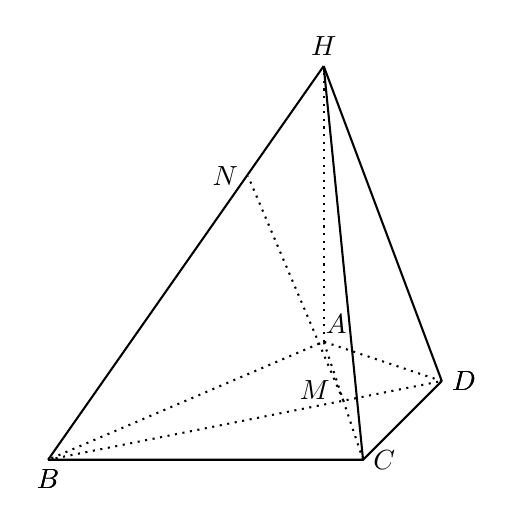
\begin{tikzpicture}
\draw [line width=0.75pt]  (0,0)node[below] {$B$} --(4,0)node[right] {$C$}--(5,1)node[right] {$D$};
\draw [dotted,line width=0.75pt] (5,1)--(3.5,1.5)--(0,0);
\draw [dotted,line width=0.75pt](3.5,1.5)--(3.5,5)node[above]{$H$};
\draw [line width=0.75pt] (3.5,5)--(4,0);
\draw [line width=0.75pt] (3.5,5)--(5,1);
\draw [line width=0.75pt] (3.5,5)--(0,0);
%\draw [dotted,line width=0pt](3.5,1.5)--(3.3,1.51)node[above]{$A$};     %被线挡,实在没办法了,只好这样标记A点
\node at (3.66,1.48) [above]{$A$};                                                                %翻了一下手册,原来node还能这么用
%\draw [white](3.5,1.5)--(3.3,1.51)node[above,color=black]{$A$};            %随后联想到颜色,果然。这仨效果完全相同
\draw [dotted,line width=0.75pt]  (0,0)node[below] {$B$} --(5,1)node[right] {$D$};
\draw [dotted,line width=0.75pt]  (4,0)--(3.5,1.5);
\node at (3.7,0.88) [left]{$M$}; 
\draw [dotted,line width=0.75pt] (3.75,0.75)--(2.54,3.6)node[left]{$N$};   %tikz一定有算法,A又被档…有时间再去翻手册,这会人工调整
\end{tikzpicture}
 %%% 用tikz画了,只用最简单的--及最简单的标ABC法,这里纯人工调整 tikz一定有别的算法 by iC %%%

\vfill



\item     已知函数$f(x) = \dfrac13x^3 + mx^2 - 3m^2x + 1,(m\in\mathbb{R})\).

(\uppercase\expandafter{\romannumeral1})当$m=1$时,求曲线\(f(x)\)在点$(2,f(2)$ 处的切线方程;

(\uppercase\expandafter{\romannumeral2})若\(f(x)\)在区间$(2m-1,m+1)$ 上单调递增,求$m$的取值范围.

\vfill



\newpage


\item     已知$M$是由满足下述条件的函数构成的集合:


对$\forall \ f(x)\in M$,\ding{192}方程$f(x)-x=0$有实数根;\ding{193}函数$f(x)$ 的导数 $f'(x)$满足$0<f'(x)<1$ .


 (\uppercase\expandafter{\romannumeral1})判断函数$f(x)=\dfrac x2 +\dfrac {\sin x}4$是否是集合$M$中的元素,并说明理由;


(\uppercase\expandafter{\romannumeral2})集合$M$中的元素$f(x)$ 具有下面的性质:

若$f(x)$ 的定义域为$D$,则对于$\forall \ [m,n]\subseteq D$,都$\exists \ x_0\in(m,n)$ ,使得等式$f(n)-f(m)=(n-m)f'(x_0)$ 成立.

试用这一性质证明:方程$f(x)-x=0$有且只有一个实数根.


\end{enumerate}
\end{document}
